\documentclass[a4paper, 14pt]{extreport}
\usepackage{cmap}
\usepackage{amssymb}
\usepackage{amsmath}
\usepackage{graphicx}
\usepackage{amsthm}
\usepackage{upgreek}
\usepackage{listings}
\usepackage{setspace}
\usepackage{booktabs}
\usepackage{array}
\usepackage{pdflscape} % Для альбомной ориентации страницы
\usepackage{makecell}
\usepackage{longtable}
\numberwithin{equation}{section}
\usepackage[T2A]{fontenc}
\usepackage[utf8]{inputenc}
\usepackage[normalem]{ulem}
\usepackage{mathtext} % русские буквы в формулах
\usepackage[left=3cm,right=1.5cm,top=2cm,bottom=2cm]{geometry}
\usepackage{linegoal}
\usepackage[english,russian]{babel}
\usepackage[unicode]{hyperref}
\usepackage{indentfirst}
\setlength{\parindent}{1cm} % Настройка длины красной строки (например, 1.25 см)
%\usepackage{pythonhighlight}

\usepackage{titlesec}
\usepackage{caption}
\usepackage{multirow}

\newcommand{\specialcell}[2][c]{%
	\begin{tabular}[#1]{@{}c@{}}#2\end{tabular}}

% Настройка заголовков для таблиц
\captionsetup[table]{labelsep=space}
\addto\captionsrussian{\renewcommand{\tablename}{\bfseries Таблица}}
% chapter settings
\titleformat{\chapter}[display]
{\centering\large\bfseries}{\chaptertitlename\ \thechapter}{0pt}{\large}   
\titlespacing*{\chapter}{5pt}{-20pt}{18pt}
\titlespacing*{\section}{0pt}{18pt}{18pt} 
\titlespacing*{\subsection}{0pt}{18pt}{18pt} 
\titlespacing*{\subsubsection}{0pt}{5pt}{5pt} 
% section settings
\titleformat{\section}[block]
{\raggedright\large\bfseries}
{\hspace{1.25cm}\thesection\ }{0pt}{}
\titleformat{\subsection}[block]
{\raggedright\large\bfseries}
{\hspace{1.25cm}\thesubsection\ }{0pt}{}
\titleformat{\subsubsection}
{\raggedright\normalfont\normalsize\bfseries} % Шрифт для подподсекции
{\thesubsubsection\hspace{0.5em}} % Номер подподсекции с пробелом
{0pt} % Отступ от номера
{\hspace{1.25cm}}
\addto\captionsrussian{% Replace "english" with the language you use
	\renewcommand{\contentsname}%
	{\centering \large ОГЛАВЛЕНИЕ}%
	\renewcommand{\chaptername}{ГЛАВА}
	\renewcommand{\chaptertitlename}{ГЛАВА}
	\renewcommand{\bibname}{\large СПИСОК ИСПОЛЬЗОВАННОЙ ЛИТЕРАТУРЫ}
}


\newcommand\Norm[1]{\left\| #1 \right\|}
\newcommand{\dif}{\mathrm{d}}
\newcommand{\Rm}{\mathbb{R}}
\newcommand{\Cm}{\mathbb{C}}
\newcommand{\Z}{\mathbb{Z}}
\newcommand{\I}{\mathbb{I}}
\newcommand{\N}{\mathbb{N}}
\newcommand{\rank}{\operatorname{rank}}
\newcommand{\Ra}{\Rightarrow}
\newcommand{\ra}{\rightarrow}
\newcommand{\FI}{\Phi}
\newcommand{\Sp}{\text{Sp}}
\renewcommand{\leq}{\leqslant}
\renewcommand{\geq}{\geqslant}

% 	КРАСИВЫЕ ГРЕЧЕСКИЕ СИМВОЛЫ
\renewcommand{\alpha}{\upalpha}
\renewcommand{\beta}{\upbeta}
\renewcommand{\gamma}{\upgamma}
\renewcommand{\delta}{\updelta}
\renewcommand{\epsilon}{\upvarepsilon}
\renewcommand{\zeta}{\upzeta}
\renewcommand{\eta}{\upeta}
\renewcommand{\theta}{\uptheta}
\renewcommand{\kappa}{\upkappa}
\renewcommand{\lambda}{\uplambda}
\renewcommand{\mu}{\upmu}
\renewcommand{\xi}{\upxi}
\renewcommand{\pi}{\uppi}
\renewcommand{\rho}{\uprho}
\renewcommand{\sigma}{\upsigma}
\renewcommand{\tau}{\uptau}
\renewcommand{\varphi}{\upvarphi}
\renewcommand{\chi}{\upchi}
\renewcommand{\psi}{\uppsi}
\renewcommand{\omega}{\upomega}

\renewcommand{\d}{\partial}


\newcommand{\cov}{\operatorname{cov}}
\newcommand{\E}{\mathbb E}
\newcommand{\corr}{\operatorname{corr}}
\newcommand{\Var}{\operatorname{Var}}
\newcommand{\const}{\operatorname{const}}
\renewcommand{\I}{\operatorname{I}}
\renewcommand{\i}{\operatorname{i}}
\newcommand{\bi}{\operatorname{bi}}
\numberwithin{equation}{section}
\newtheorem*{theorem}{Теорема}
\newtheorem*{cor}{Следствие}
\newtheorem*{lem}{Лемма}
\usepackage{stackengine}

% Переоформление некоторых стандартных названий

\begin{document}
	\def\contentsname{ОГЛАВЛЕНИЕ}
	
	\def\contentsname{ОГЛАВЛЕНИЕ}
	
	\begin{titlepage}
		\begin{center}
			\textbf{БЕЛОРУССКИЙ ГОСУДАРСТВЕННЫЙ УНИВЕРСИТЕТ
				\\[5mm]
				{ФАКУЛЬТЕТ ПРИКЛАДНОЙ МАТЕМАТИКИ И ИНФОРМАТИКИ}\\[2mm]
				Кафедра математического моделирования и анализа данных
			}
			
			\vfill
			
			\textbf{Отчет
				\\[3mm]
				о прохождении производственной (преддипломной) практики
				\\[26mm]
			}
		\end{center}
		
		\hfill
		\begin{minipage}{.7\textwidth}
			\begin{flushright}
				Бовта Тимофея Анатольевича\\
				студента 4 курса 7 группы\\
				специальности «Прикладная математика»\\[5mm]
				
				Руководитель практики:\\[2mm] 
				зав. кафедрой математического моделирования\\
				и анализа данных ФПМИ,\\
				доктор экономических наук,\\
				кандидат физико-математических наук,\\
				профессор В.И. Малюгин
				
				
			\end{flushright}
		\end{minipage}
		\vfill
		\begin{center}
			Минск, 2025\ г.
		\end{center}
	\end{titlepage}
	\newpage
	\setcounter{page}{2}
	\begin{center}
		{
			\setstretch{0.5}
			\mbox{БЕЛОРУССКИЙ~ГОСУДАРСТВЕННЫЙ~УНИВЕРСИТЕТ} \\~\\
			\mbox{Факультет~прикладной математики~и~информатики} \\~\\
			\mbox{Кафедра~математического~моделирования~и~анализа~данных} \\~\\[2mm]
		}
		\vspace{0.5cm}
		\hfill
		\begin{minipage}{.6\textwidth}
			\begin{flushright}
				\textbf{Утверждаю}\hspace*{4.2cm} \\
				Заведующий кафедрой \underline{\hspace*{4cm}}\\[-2mm]
				{\scriptsize(подпись)(фамилия, инициалы)}\\[2ex]
				«\underline{\hspace*{0.5cm}}»\underline{\hspace*{2cm}}20\underline{\hspace*{0.5cm}}г.
				
			\end{flushright}
		\end{minipage}
		
		\vspace{1cm}
		\bf
		{
			\mbox{Задание на практику}\\
			\mbox{по специальности «Прикладная математика»} \\[6mm]
		}
	\end{center}
	Студенту Бовту Т. А.\\[2mm]
	1. Тема практики:
	<<Краткосрочное прогнозирование и наукастинг макроэкономических временных рядов на основе векторных моделей авторегрессии по смешанным данным>>.\\[6mm]
	2. Список рекомендуемой литературы:
	
	2.1. Малюгин В. И. Краткосрочное прогнозирование и наукастинг темпов роста инфляции на основе моделей по смешанным данным --- Журнал <<Банковский вестник>> №1/726 --- С. 23-36.
	
	2.2. Макеева, Н.М. Наукастинг элементов использования ВВП России / Н.М. Макеева, И.П. Станкевич -- Статья 2022/10, Экономический журнал ВШЭ.
	
	2.3. Макеева, Н.М. Наукастинг макроэкономических показателей экономики России на основе анализа новостного фона и регулярных данных Росстата / Н. М. Макеева, И. П. Станкевич\\[6mm]
	3. Перечень подлежащих разработке вопросов или краткое содержание
	расчетно-пояснительной записки:
	
	3.1. подготовка обзора основных многомерных подходов, применяемых для краткосрочного прогнозирования;
	
	3.2. описание математических моделей и методов их построения, используемых для решения задачи прогнозирования ВВП Республики Беларусь;
	
	3.3. построение соответствующих моделей для прогнозирования;
	
	3.4. сравнительный анализ моделей по смешанным данным с моделями по агрегированным данным;
	
	3.5. подготовка отчета и презентации по выполненной работе.\\[6mm]
	4. Примерный календарный график:\\[6mm]
	
	-- \textbf{февраль (1-ая неделя)} -- получение задания, загрузка новых данных для исследования; изучение функции импульсных откликов для VAR модели;
	
	-- \textbf{февраль (2-3-я неделя)} -- изучение функции спроса на деньги, сбор статистик по ВВП, инфляции, ставке, моделирование денежной массы; изучение понятия эластичности в экономике, основных статистических методов работы с экономическими данными;
	
	-- \textbf{март (4-5-ая неделя)} -- изучение основных методов расчета ВВП, изучение экономических взаимосвязей между ВВП и опережающими показателями; исследование показателя СИЭН, его взаимосвязи с ВВП; построение плана оформления I-III глав дипломной работы;
	
	-- \textbf{март (6-7-ая неделя)} -- написание отчета по теоретическим взаимосвязям модели ВВП и статистическому анализу временных рядов; программирование алгоритма расширяющегося окна; построение модели ВВП; оценка точности прогнозов;
	
	-- \textbf{апрель (8-9-ая неделя)} -- составление плана IV главы в дипломной работе; общая характеристика модели ВВП белорусской экономики; написание IV главы, сравнительный анализ построенных моделей;
	
	
	-- \textbf{апрель (10-ая неделя)} -- оформление отчета по проделанной работе; интерпретация полученных результатов.\\[6mm]
	5. Руководители практики:
	
	от предприятия Демиденко Михаил Витальевич;
	
	от кафедры Малюгин Владимир Ильич.\\[6mm]
	6. Дата выдачи задания 10.02.2025.\\[6mm]
	7. Срок сдачи отчета\hspace*{0.7cm} 21.04.2025.\\[10mm]
	Руководитель \underline{\hspace*{4cm}} В.И.Малюгин\\[-2mm]
	{\scriptsize(от кафедры)\hspace*{1.5cm}(подпись)}\\[2ex]
	\noindent Подпись студента \underline{\hspace*{6cm}} \\[-2mm]
	{\scriptsize\hspace*{6cm}(подпись, дата)}\\[2ex]
	\newpage
	
	
	% Содержание
	\tableofcontents
	\newpage
	\chapter*{\centering ВВЕДЕНИЕ}\addcontentsline{toc}{chapter}{ВВЕДЕНИЕ}
	Отдельные фундаментальные макроэкономические показатели формируются Национальным статистическим комитетом Республики Беларусь на квартальной и годовой частоте. В то же время доступны более оперативные показатели, которые публикуются с месячной и дневной периодичностью.
	В частности, показатель внутреннего валового продукта (ВВП) по методу использования доходов формируется на квартальной частоте, а отраслевые показатели и статистика цен – на месячной частоте, обменные курсы валют и денежно-кредитные показатели – на дневной частоте. 
	Причем в соответствии с Регламентом публикации данных оценок ВВП Республики Беларусь квартальная оценка ВВП публикуется на 90-ый день после окончания отчетного квартала. В связи с этим становится актуальным вопрос об использовании более оперативной информации при прогнозировании показателя ВВП.
	
	Все классические регрессионные модели машинного обучения работают с данными, заданными на одной частоте.  Соответственно в ходе предварительного анализа приходится преобразовывать данные к одной частоте. Как правило, выбирается один из следующих способов.
	\begin{enumerate}
		\item \textit{Агрегация данных высокой частоты. }
		
		\item \textit{Интерполяция низкочастотных
			переменных.}
	
	\end{enumerate}
	
	Таким образом, вопрос о том, как можно без преобразования данных и потери какой-либо информации строить регрессионную модель для моделирования исследуемых показателей, становится актуален.
	
	В данной работе для решения задачи моделирования показателя ВВП Республики Беларусь, представленного на квартальной частоте, по опережающим факторам на месячной частоте рассматриваются специальные регрессионные модели, предназначенные для работы с данными смешанной частоты -- MFVAR (Mixed Frequency Vector Autoregression). В последнее время эти модели используются для прогнозирования макроэкономических временных рядов, где обычно квартальный
	рост ВВП прогнозируется по месячным макроэкономическим и финансовым показателям. Разработка моделей, способных работать с переменными, отбираемыми на разной частоте вызывает значительный интерес в сфере эконометрии.
	
	В отличие от одномерных регрессионных моделей, векторные авторегресиионные модели позволяют не только установить характер зависимости эндогенного показателя от экзогенных, но и понять, как в целом построена связь между всеми переменными в системе и их поведением в прошлом.
	
	\newpage
	\chapter{СТАТИСТИЧЕСКИЙ АНАЛИЗ МАКРОЭКОНОМИЧЕСКИХ ВРЕМЕННЫХ РЯДОВ}
	\section{Математическое описание исследуемых экономических показателей}
	
	Для проведения исследований нам даны следующие экономические показатели, для которых мы введем краткие обозначения
	\begin{itemize}
		\item квартальная частота:
		\begin{itemize}
			\item rGDP\_q $:= Y_t^Q$ -- реальный ВВП Беларуси по источникам использования доходов в среднегодовых ценах 2018 г., млн. руб.;
		\end{itemize}
		\item месячная частота:
		\begin{itemize}
			\item rPP\_m $:= IP_t^M$ -- объем промышленного производства в среднегодовых ценах 2018 г., млн. руб.;
			\item rRet\_m $:= RT_t^M$ -- объем розничного товарооборота в среднегодовых ценах 1995 г., млн. руб.;
			\item rInv\_m $:=INV_t^M$ -- объем инвестиций в основной капитал в среднегодовых ценах 2018 г., млн. руб.;
			\item rAgro\_m $:=AGRO_t^M$ -- объем продукции сельского хозяйства в среднегодовых ценах 2018 г., млн. руб.;
			\item Bi\_Bld\_m $:=\bi BLD_t^M$ -- базисный индекс объема строительно монтажных работ (янв. 2018 = 1), \%;
			\item Bi\_rRdh\_m $:=\bi INC_t^M$ -- базисный индекс объема денежных доходов населения (янв. 2018 = 1). \%;
			\item CESI\_m\_SA $:=CESI_t^{M*}$-- сезонно-скорректированный сводный индекс экономических настроений.
		\end{itemize}
	\end{itemize}
	
	Период наблюдения данных следующий
	\begin{itemize}
		\item для квартальных: 1 квартал 2009 года — 1 квартал 2025 года;
		\item для месячных: 1 месяц 2009 года — 1 месяц 2025 года.
	\end{itemize}
	
	Авторегрессионные модели корректно работают со стационарными временными рядами, поскольку все они строились именно для стационарных рядов. Следовательно, необходимо определить, являются ли данные временные ряды стационарными. И если они не являются стационарными, то необходимо привести их к стационарному виду, чтобы получить качественные результаты прогнозирования.
	
	Для того, чтобы определить алгоритм приведения рядов к стационарному виду, рассмотрим графики исходных рядов (Рисунок \ref{fig:ts-1}).
	
	\begin{figure}[h!]
		\centering
		\begin{minipage}{0.5\textwidth}
			\centering
			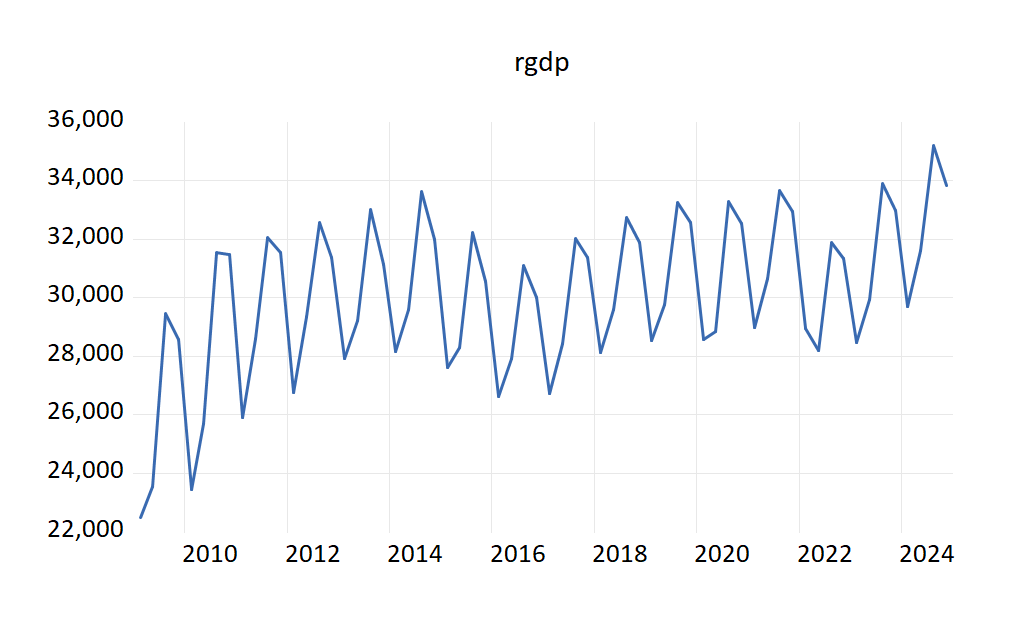
\includegraphics[scale=0.4]{images/image05}
			\caption*{а)}
		\end{minipage}%
		\begin{minipage}{0.5\textwidth}
			\centering
			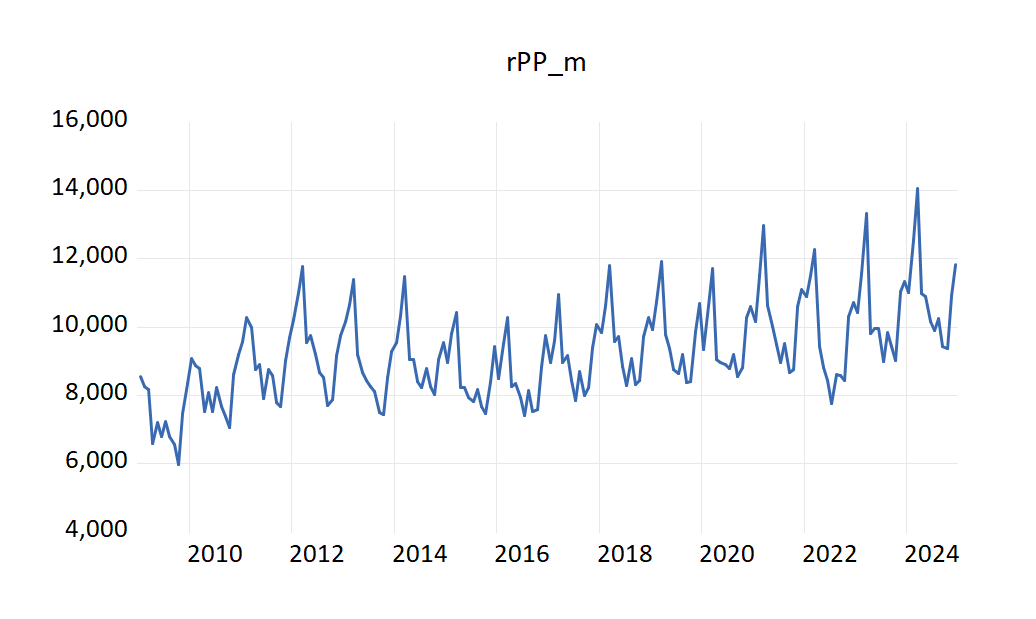
\includegraphics[scale=0.4]{images/image06}
			\caption*{б)}
		\end{minipage}%
		
		\begin{minipage}{0.5\textwidth}
			\centering
			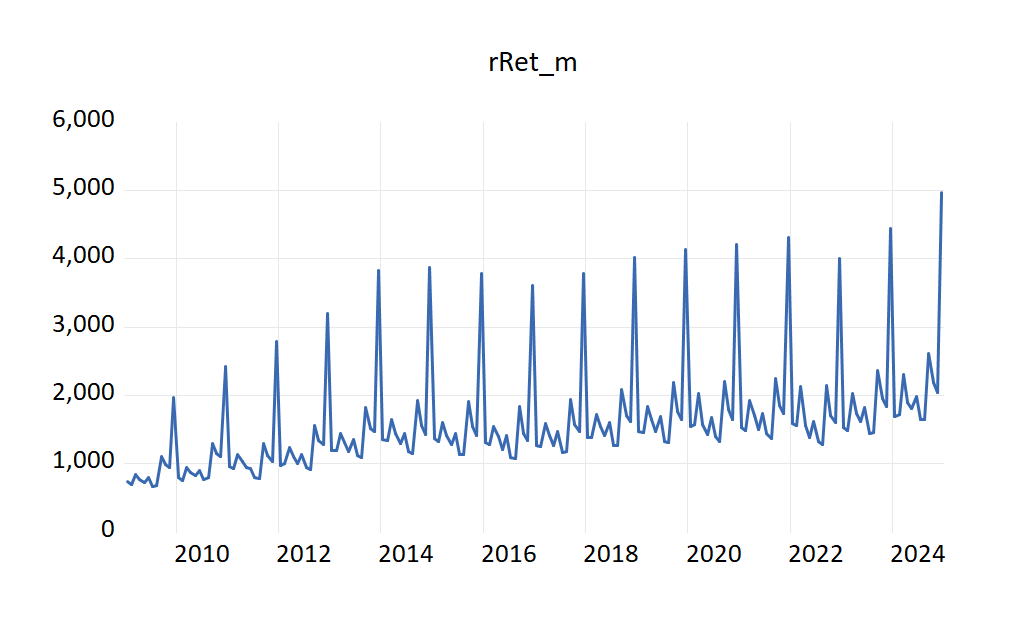
\includegraphics[scale=0.4]{images/image07}
			\caption*{в)}
		\end{minipage}%
		\hfill % Добавляем горизонтальное пространство
		\begin{minipage}{0.5\textwidth}
			\centering
			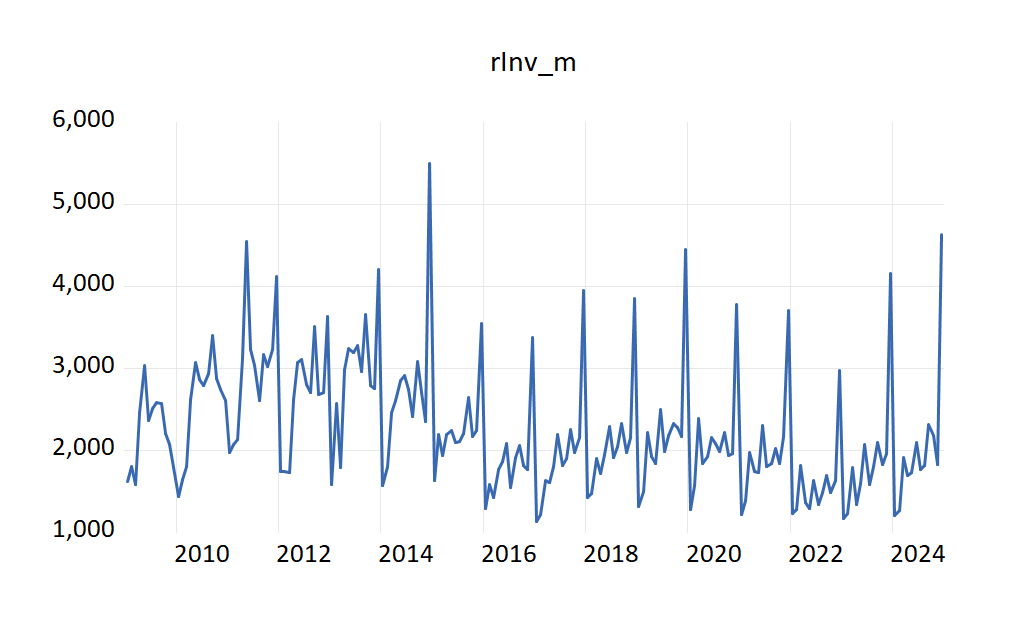
\includegraphics[scale=0.4]{images/image08}
			\caption*{г)}
		\end{minipage}%
		
		\begin{minipage}{0.5\textwidth}
			\centering
			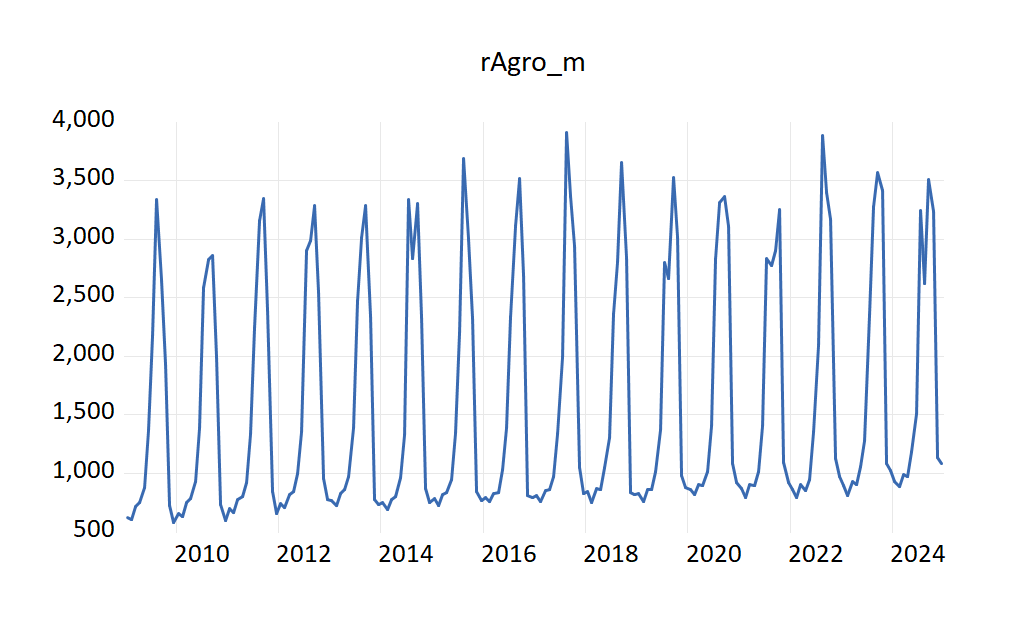
\includegraphics[scale=0.4]{images/image09}
			\caption*{д)}
		\end{minipage}%
		\hfill % Добавляем горизонтальное пространство
		\begin{minipage}{0.5\textwidth}
			\centering
			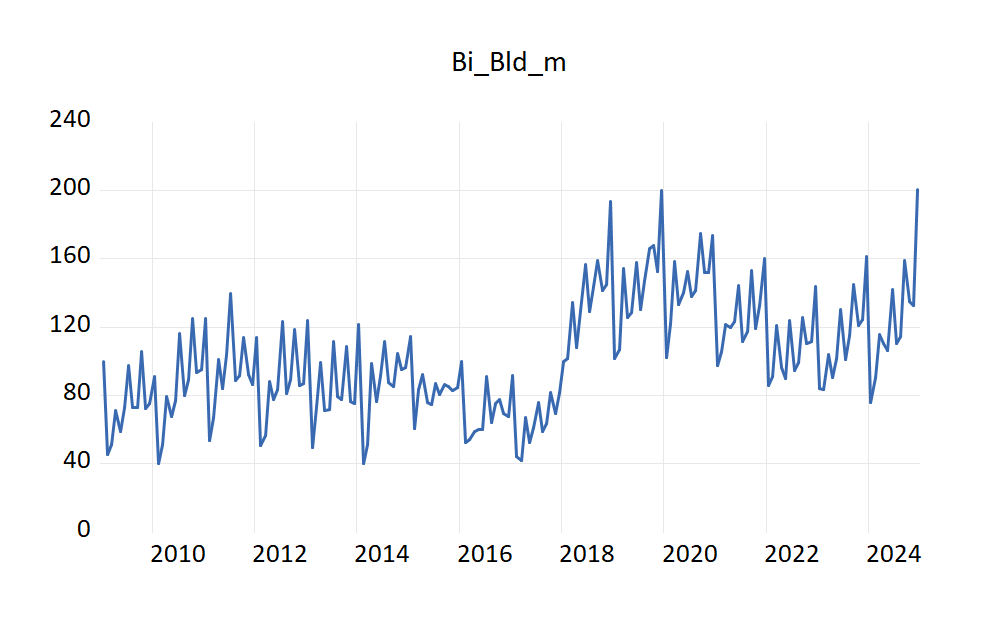
\includegraphics[scale=0.4]{images/image10}
			\caption*{е)}
		\end{minipage}
		
		\begin{minipage}{0.5\textwidth}
			\centering
			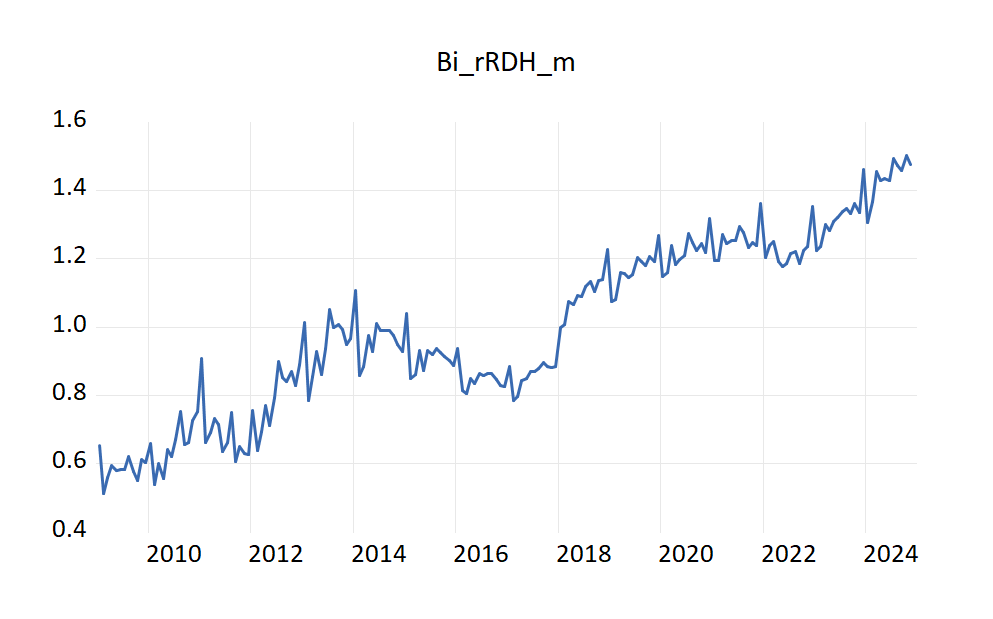
\includegraphics[scale=0.4]{images/image12}
			\caption*{ж)}
		\end{minipage}%
		\hfill % Добавляем горизонтальное пространство
		\begin{minipage}{0.5\textwidth}
			\centering
			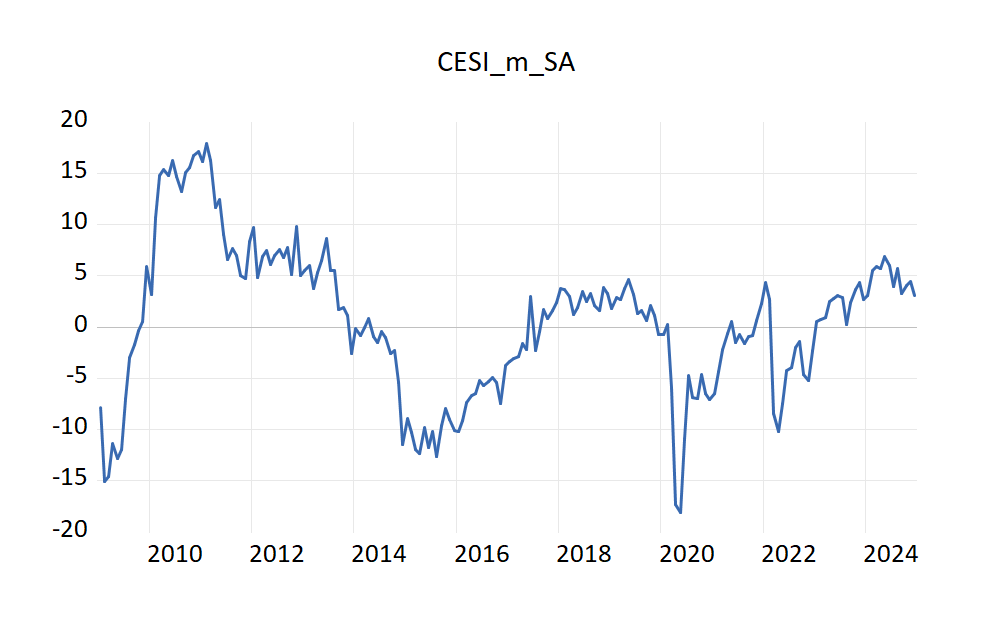
\includegraphics[scale=0.4]{images/image14}
			\caption*{з)}
		\end{minipage}
		
		\caption{\centering --- Исходные ряды: а) {$Y_t^Q$}; б) {$IP_t^M$}; в) {$RT_t^M$};\\ г) {$INV_t^M$}; д) {$AGRO_t^M$}; е) {$\bi BLD_t^M$}; ж) $\bi INC_t^M$; з) $CESI^{M*}_t$.}
		\label{fig:ts-1}
	\end{figure}
	
	Из графиков временных рядов заметно, что они все кроме СИЭН обладают сезонным эффектом. Следовательно, сперва необходимо провести сезонную корректировку.

	Прогнозируемый временной ряд ВВП мы будем рассматривать в темпах прироста год к году, что само по себе является сезонной корректировкой. 
	
	Исключим сезонную компоненту из временных рядов $IP_t^M$, $RT_t^M$, $INV_t^M$, $AGRO_t^M$, $\bi BLD_t^M$,  $\bi INC_t^M$ с помощью метода TRAMO/SEAT.
	Применяя последовательно этот метод к каждому из рассматриваемых временных рядов, мы получим временные ряды без сезонной компоненты. 
	
	Во временных рядах без сезонной компоненты присутствует трендовая компонента. Сперва перейдем от сезонно скорректированных временных рядов к логарифмическим, чтобы заменить экспоненциальный рост линейным.
	После чего возьмем темпы прироста в логарифмах, чтобы привести все временные ряды к процентной шкале. Причем в месячных временных рядах кроме СИЭН перейдем к темпам прироста месяц к месяцу, а в квартальном ВВП -- год к году. 
	
	Полученные временные ряды изображены на Рисунке \ref{fig:ts-3}. 
	
	\begin{figure}[h!]
		\centering
		\begin{minipage}{0.5\textwidth}
			\centering
			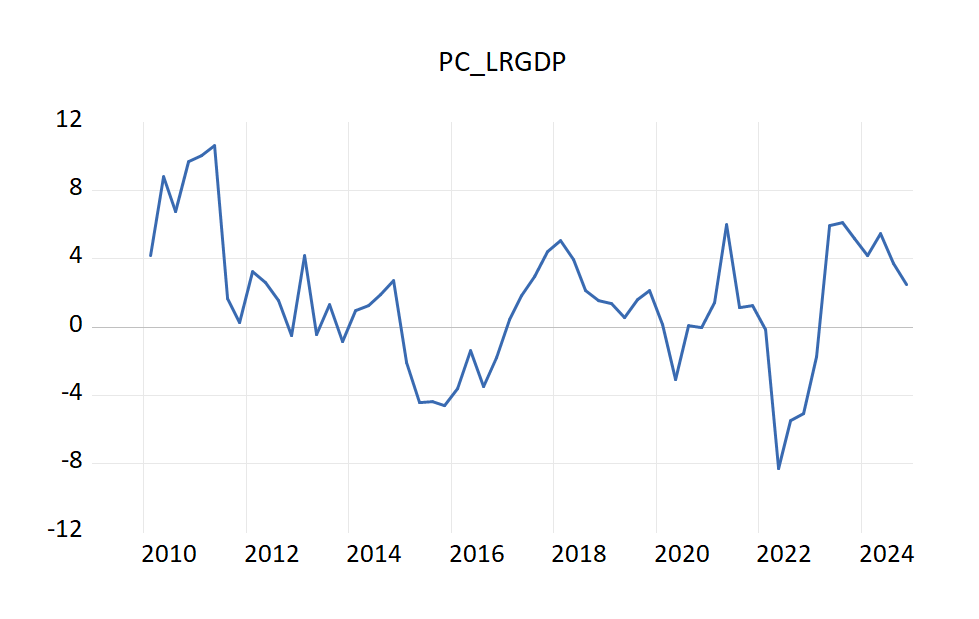
\includegraphics[scale=0.4]{images/image22}
			\caption*{а)}
		\end{minipage}%
		\begin{minipage}{0.5\textwidth}
			\centering
			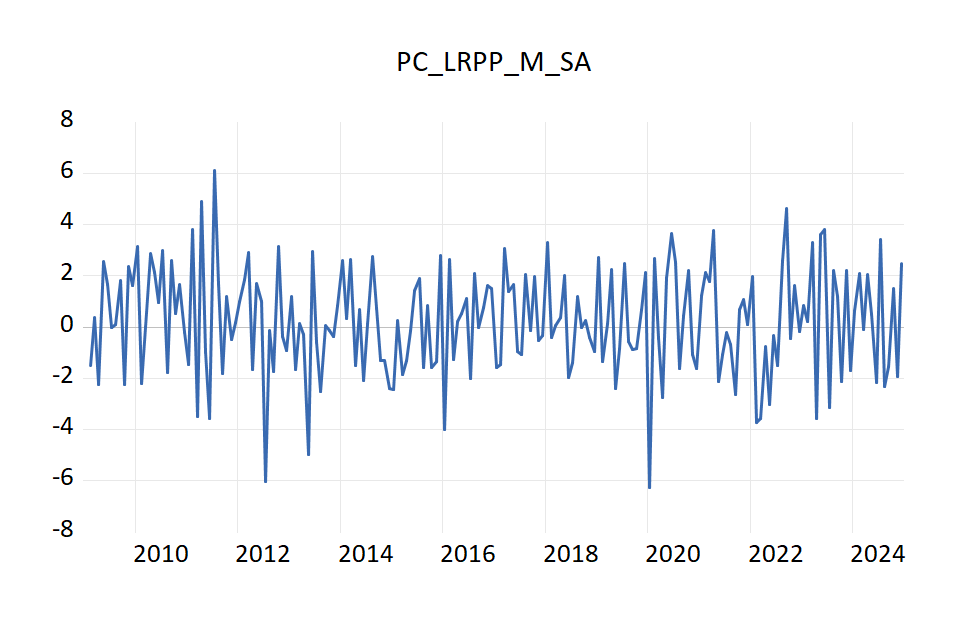
\includegraphics[scale=0.4]{images/image23}
			\caption*{б)}
		\end{minipage}%
		
		\begin{minipage}{0.5\textwidth}
			\centering
			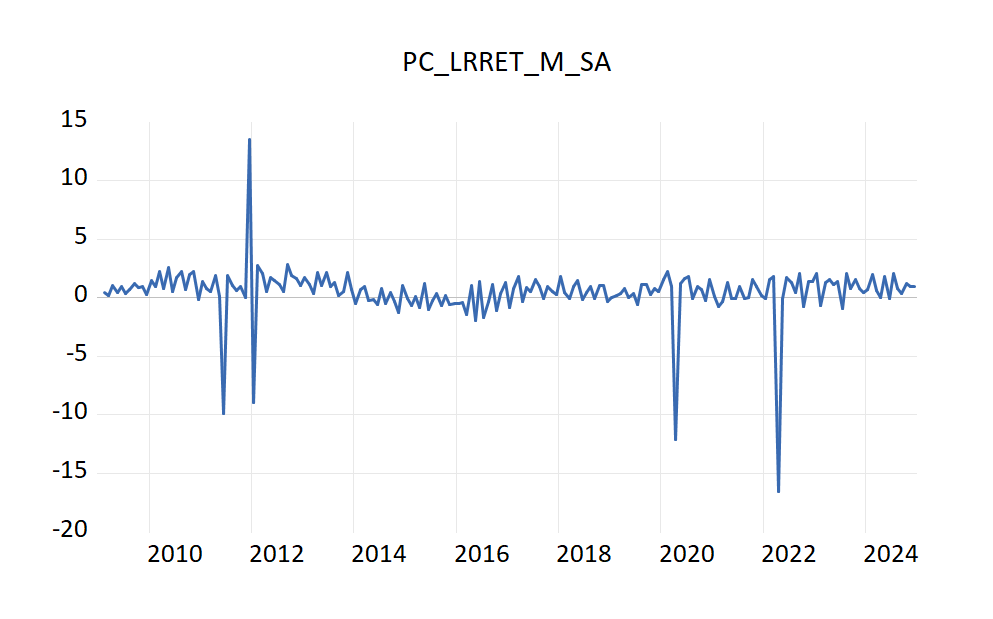
\includegraphics[scale=0.4]{images/image24}
			\caption*{в)}
		\end{minipage}%
		\hfill % Добавляем горизонтальное пространство
		\begin{minipage}{0.5\textwidth}
			\centering			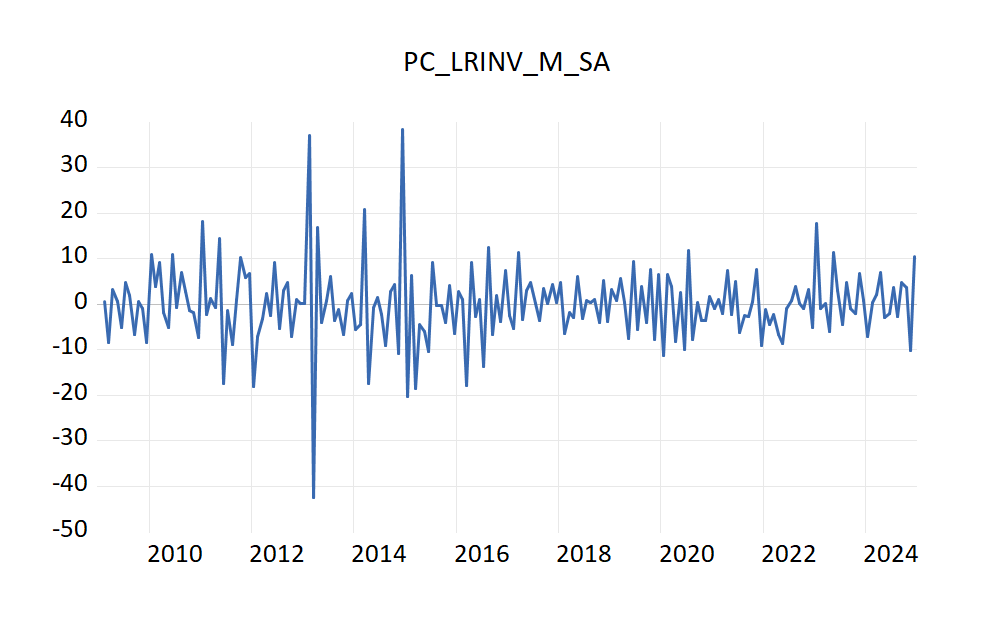
\includegraphics[scale=0.4]{images/image25}
			\caption*{г)}
		\end{minipage}%
		
		\begin{minipage}{0.5\textwidth}
			\centering
			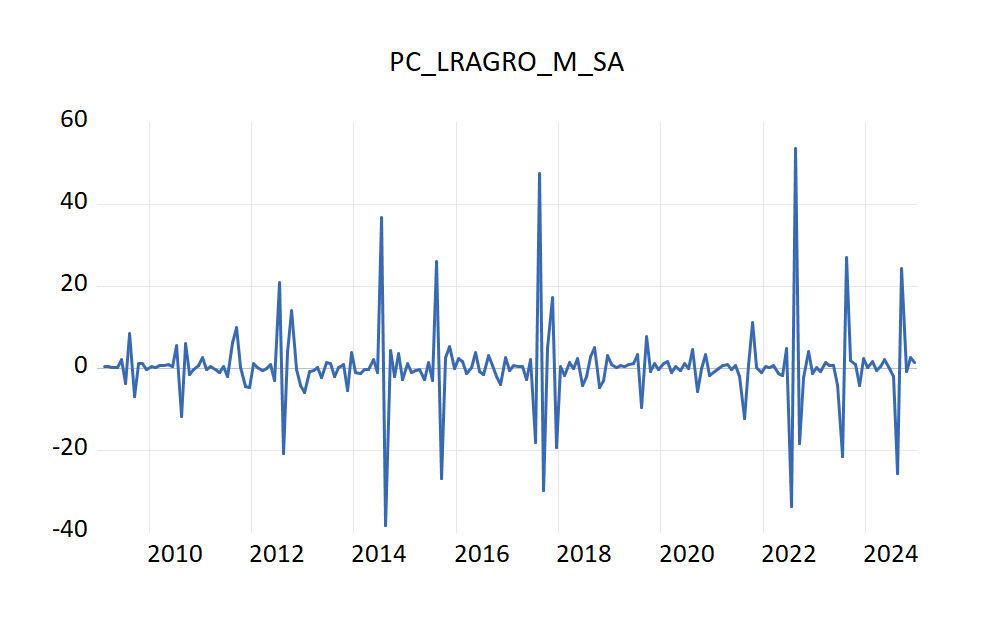
\includegraphics[scale=0.4]{images/image26}
			\caption*{д)}
		\end{minipage}%
		\hfill % Добавляем горизонтальное пространство
		\begin{minipage}{0.5\textwidth}
			\centering
			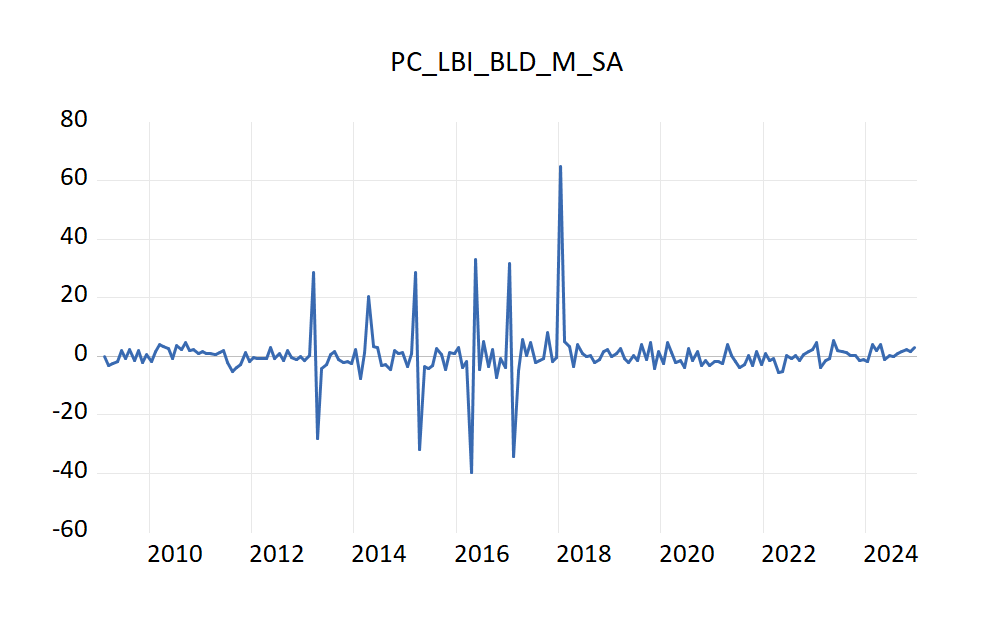
\includegraphics[scale=0.4]{images/image27}
			\caption*{е)}
		\end{minipage}
		
		\begin{minipage}{0.5\textwidth}
			\centering
			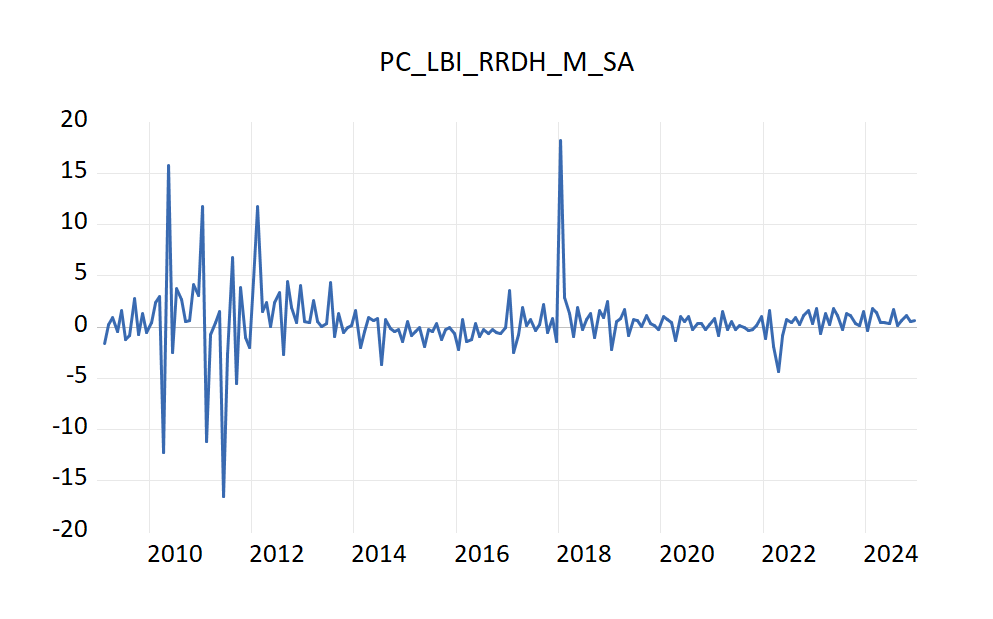
\includegraphics[scale=0.4]{images/image28}
			\caption*{ж)}
		\end{minipage}%
		\hfill % Добавляем горизонтальное пространство
		\begin{minipage}{0.5\textwidth}
			\centering
			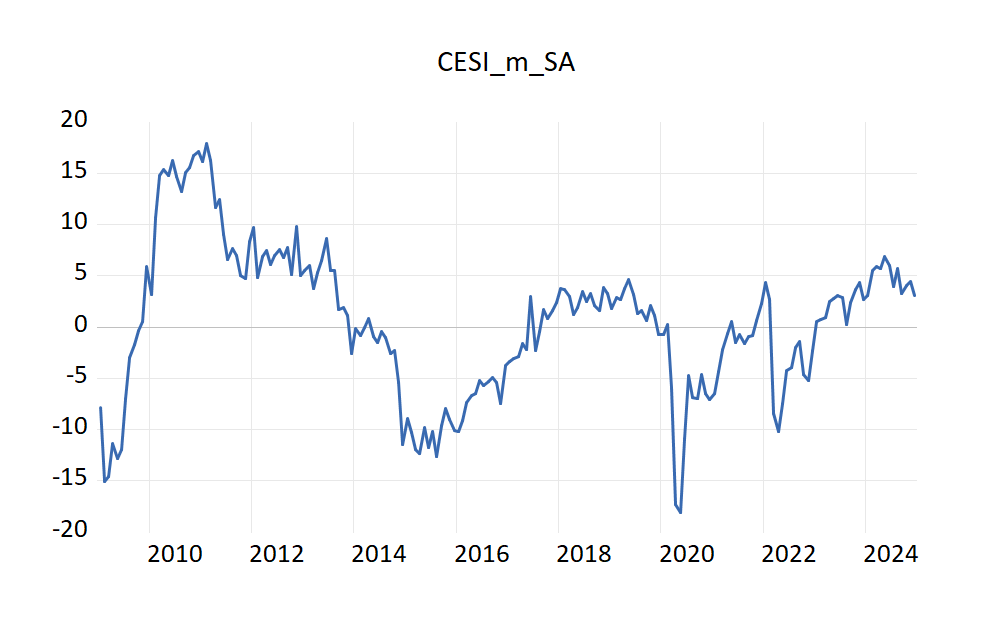
\includegraphics[scale=0.4]{images/image14}
			\caption*{з)}
		\end{minipage}
		
		\caption{\centering --- Ряды темпов прироста в логарифмах: а) $\i y_t^Q$; б) $\i ip_t^{M*}$;\\ в) $\i rt_t^{M*}$; г) $\i inv_t^{M*}$; д) $\i agro_t^{M*}$; е) $\i \bi bld_t^{M*}$; ж) $\i \bi inc_t^{M*}$; з) $CESI^{M*}_t$.}
		\label{fig:ts-3}
	\end{figure}
	
	Таким образом, временной ряд $\i y_t^Q$ отражает темпы прироста продукции в логарифмах в текущем квартале по отношению к соответствующему кварталу предыдущего года. Остальные ряды отражают темпы прироста в логарифмах текущего месяца к предыдущему месяцу. Важно понимать, что темпы прироста в логарифмах не совпадают с реальными рядами темпов прироста, а являются аппроксимацией. Однако принято считать эту аппроксимацию достаточно точной, чтобы использовать ее.
	
	
	
	В итоге мы получили новые временные ряды, в которых отсутствуют трендовая и сезонная компоненты. 
	
	Визуально можно предположить, что полученные ряды являются стационарными, так как все они явно колеблются около нуля с некоторым постоянным отклонением. Это предположение также соответствует экономическому смыслу: в силу того, что темпы прироста показателя -- это процентное изменение в текущем периоде относительно предыдущего периода, то в среднем ожидается прирост 0\%, то есть показатель останется на том же уровне. Индекс СИЭН выражен не в темпах прироста, однако имеет схожий экономический смысл. Поскольку он является линейной комбинацией из ответов менеджеров вида << + >>, << 0 >>, << - >>, то в среднем также ожидается, что в текущем опросном периоде экономические настроения останутся на том же уровне, что и в предыдущем.
	
	Необходимо также статистически подкрепить предположения о стационарности полученных рядов. 
	
	\section{Тестирование стационарности}
	Для тестирования временных рядов на стационарность используется расширенный тест Дики-Фуллера.
	Этот тест является стандартным инструментом анализа временных рядов, однако следует отметить, что он может быть склонен к ошибочным выводам в случаях наличия структурных изменений.
	В связи с этой проблемой мы также применим модифицированный ADF-тест, известный как Break Point Unit Root (BPUR-тест). Этот тест позволяет выявить одно наиболее выраженное структурное изменение во временном ряде, описываемом DS-моделью, что делает его полезным инструментом для более точного анализа.
	
	Для определенности количество лагов в модели ADF-теста будет выбираться основе информационного критерия Шварца.
	
	\begin{table}[h!]
		\centering
		\caption{\label{adf-bpur} -- Результаты тестирования на единичный корень с помощью ADF-теста без константы и BPUR-теста с AO}
		\label{table:ADF-BPUR-test}
		\begin{tabular}{|l|c|c|c|c|c|c|}
			\hline
			\multirow{2}{*}{\makecell{\textbf{Пере-} \\ \textbf{менные}}} & \multicolumn{3}{c|}{\textbf{ADF-тест}} & \multicolumn{3}{c|}{\textbf{BPUR-тест}} \\ \cline{2-7}
			& \makecell{t-\\ADF} & \makecell{$p$-\\значение} & \makecell{H\textsubscript{0}: \\ единичный \\ корень} & \makecell{t-\\ADF} & \makecell{$p$-\\значение} & \makecell{H\textsubscript{0}: \\ единичный \\ корень} \\ \hline
			$\i y_t^Q$ & -2.80 & 0.006 & отвергается & -4.49 & 0.045 &  отвергается \\ \hline
			$\i ip_t^{M^*}$ & -17.24 & 0.000 & отвергается & -18.21 & $<$ 0.01 &  отвергается \\ \hline
			$\i rt_t^{M^*}$ & -15.52 & 0.000 & отвергается & -19.11 & $<$ 0.01 &  отвергается \\ \hline
			$\i inv_t^{M^*}$ & -23.56 & 0.000 & отвергается & -24.33 & $<$ 0.01 &  отвергается \\ \hline
			$\i agro_t^{M^*}$ & -11.35 & 0.000& отвергается & -25.94 & $<$ 0.01 &  отвергается \\ \hline
			$\i \bi bld_t^{M^*}$ & -17.64 & 0.000 & отвергается & -18.97 & $<$ 0.01 &  отвергается \\ \hline
			$\i \bi inc_t^{M^*}$ & -16.23 & 0.000 & отвергается & -18.13 & $<$ 0.01 &  отвергается \\ \hline
			$CESI_t^{M^*}$ & -2.52 & 0.012 & отвергается & -3.42 & 0.429 & не отвергается \\ \hline
		\end{tabular}
	\end{table}
	
	
	Результаты обоих тестов позволяют отклонить гипотезу о нестационарности для всех рядов кроме индекса СИЭН; один из тестов позволяет отклонить гипотезу о нестационарности СИЭН. Однако, несмотря на то, что BPUR-тест позволяет принять гипотезу о нестационарности, мы отклоняем гипотезу в силу экономического смысла этого ряда. Следовательно, построенные временные ряды обладают всеми свойствами стационарных рядов:
	\begin{enumerate}
		\item стационарные ряды имеют постоянное среднее значение (в нашем случае равное нулю) и дисперсию;
		\item стационарные ряды позволяют использовать регрессионные модели временных рядов, включая MFVAR, без необходимости их трансформации;
		\item стационарные ряды обеспечивают более надежные прогнозы благодаря предсказуемости их поведения;
		\item стационарные ряды предполагают стабильность взаимосвязей между переменными, что важно для интерпретации результатов векторных авторегрессий.
	\end{enumerate}
	
	\newpage
	
	\chapter{МОДЕЛИРОВАНИЕ И ПРОГНОЗИРОВАНИЕ ТЕМПОВ РОСТА ВВП БЕЛАРУСИ ПО ИСТОЧНИКАМ ДОХОДОВ}
	\section{Постановка прикладной задачи}
	Национальным Банком Республики Беларусь сформулирована следующая прикладная задача по моделированию белорусской экономики. Необходимо построить математическую модель роста квартального ВВП Республики Беларусь по опережающим месячным показателям, провести прогноз с помощью этой модели и построить оценки для этого прогноза. 
	
	В таблице \ref{tab:variables} приведены все переменные, которые будут участвовать в построении математической модели
	
	\begin{longtable}{|m{3cm}|m{4cm}|m{3cm}|m{5cm}|}
		\caption{Переменные и календарь их выхода}
		\label{tab:variables} \\ 
		\hline
		\textbf{Переменная} & \textbf{Обработка} & \textbf{Описание} & \textbf{Календарь выхода} \\ 
		\hline
		$\i y_t^{Q}$ & Сезонная корректировка, темпы прироста год к году в логарифмах & Реальный ВВП Беларуси по источникам использования доходов в среднегодовых ценах 2018 г. &
		Задержка 90 дней после квартального периода + корректировка в декабре года, следующего за отчетным \\ 
		\hline
		$\i ip_t^{M*}$ & Сезонная корректировка, темпы прироста месяц к месяцу в логарифмах & Объем промышленного производства в среднегодовых ценах, 2018 г. &
		Задержка 17 дней после месячного периода \\ 
		\hline
		$\i rt_t^{M*}$ & Сезонная корректировка, темпы прироста месяц к месяцу в логарифмах & Объем розничного товарооборота в среднегодовых ценах 1995 г. &
		Задержка 18 дней после месячного периода \\ 
		\hline
		$\i inv_t^{M*}$ & Сезонная корректировка, темпы прироста месяц к месяцу в логарифма & Объем инвестиций в основной капитал в среднегодовых ценах 2018 г. &
		Задержка 24 дня после месячного периода \\ 
		\hline
		$\i agro_t^{M*}$ & Сезонная корректировка, темпы прироста месяц к месяцу в логарифма & Объем продукции сельского хозяйства в среднегодовых ценах 2018 г. &
		Задержка 19 дней после месячного периода \\ 
		\hline
		$\i \bi bld_t^{M*}$ & Сезонная корректировка, темпы прироста месяц к месяцу в логарифма & Базисный индекс объема строительно монтажных работ (янв. 2018 = 1) &
		Задержка 21 день после месячного периода \\ 
		\hline
		$\i \bi inc_t^{M*}$ & Сезонная корректировка, темпы прироста месяц к месяцу в логарифма & Базисный индекс объема денежных доходов населения (янв. 2018 = 1) &
		Задержка 30 дней после месячного периода \\
		\hline
		$CESI_t^{M*}$ & Сезонная корректировка & Сводный индекс экономических настроений &
		Задержка 4 дня после месячного периода \\
		\hline
	\end{longtable}
	
	\section{Теоретическое описание модели ВВП}
	
	Математическая модель ВВП включает два блока переменных:
	\begin{itemize}
		\item эндогенные переменные на высокой частоте (квартальной);
		\item экзогенные переменные на низкой частоте (месячной).
	\end{itemize}
	
	Всего в модели ВВП имеется $8$ переменных:
	\begin{itemize}
		\item одна эндогенная переменная на низкой частоте;
		\item семь экзогенных переменных на высокой частоте.
	\end{itemize}
	Теоретически модель ВВП можно представить в виде схемы (Рисунок \ref{fig:image41}).
	\begin{figure}[h!]
		\centering
		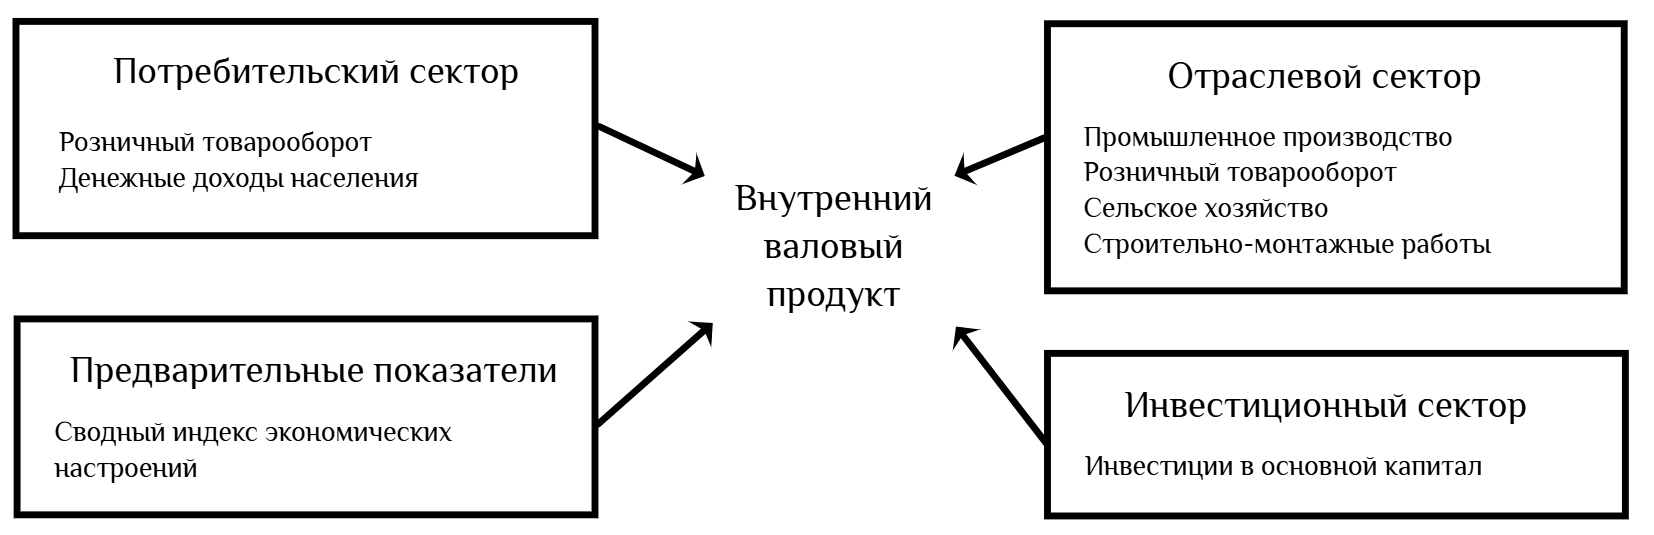
\includegraphics[scale=0.35]{images/image41}
		\caption{Схема теоретических связей в модели ВВП}
		\label{fig:image41}
	\end{figure}
	То есть модель ВВП строится по трем секторам экономики Беларуси, а также по одному предварительному показателю. 
	
	Строить математическую модель ВВП мы будем на основе векторной авторегрессии по данным смешанной частоты (MFVAR):
	\begin{itemize}
		\item  модель MFVAR представляет каждую переменную на месячной частоте в виде трех переменных на квартальной частоте;
		\item все переменные в векторных авторегрессионных моделях являются эндогенными.
	\end{itemize}
	Следовательно, каждая из семи экзогенных переменных на высокой частоте раскладывается в три переменные на низкой частоте, и мы получаем двадцать одну эндогенную переменную на низкой частоте.
	
	Также все регрессионные модели включают константу, которая соответствует отклонению значений модели от нуля. Следовательно, в MFVAR модель ВВП также добавляется экзогенная переменная на низкой частоте, которая обычно обозначается через $c$.
	
	Мы моделируем не сам временной ряд ВВП, а темпы прироста ВВП. Рассмотрим отдельно график этого временного ряда (Рисунок \ref{fig:image42}).
	\begin{figure}[h!]
		\centering
		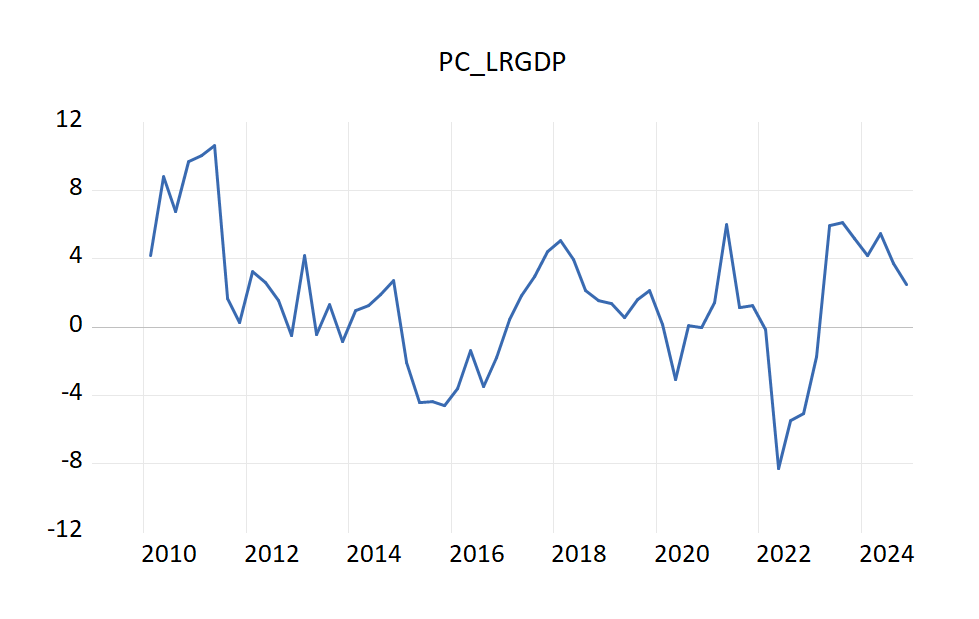
\includegraphics[scale=0.7]{images/image42}
		\caption{Темпы прироста квартал к кварталу сезонно-скорректированного ВВП}
		\label{fig:image42}
	\end{figure}
	Заметно, что во втором квартале 2022-ого года во временном ряде присутствует аномальный скачок. В силу того, что это мгновенный структурный сдвиг, модель не сможет адекватно спрогнозировать такое поведение временного ряда. Поэтому в модель включается также фиктивная переменная (dummy variable), которая будет <<подсказывать>> модели, что в этой точке происходит структурный сдвиг. Фиктивная экзогенная переменная dum2022q2 задана на квартальной частоте таким образом, что в точке 2022Q2 она принимает значение <<$1$>>, а во всех остальных точках -- <<$0$>>.
	
	Таким образом, в силу описанных условий, модель ВВП на основе MFVAR будет включать $24$ переменные:
	\begin{itemize}
		\item двадцать две эндогенные переменные на низкой частоте;
		\item две экзогенные переменных на низкой частоте.
	\end{itemize}
	Следовательно, в общем случае модель представляется в виде системы из $22$ уравнений, соответствующих каждой из эндогенных переменных.
	
	\section{Описание практической реализации модели}
	\label{sec:pract-realise}
	
	Математическая модель ВВП на основе MFVAR будет задаваться в следующем виде
	\begin{equation}
		\label{eq:mfvar-1}
		\mathbf X_t = \mathbf c + \mathbf c_1 \times \operatorname{dum2022q2} + \sum_{k=1}^{p}\mathbf B_k \times \mathbf X_{t-k} + \mathbf \epsilon_t,
	\end{equation}
	где
	$\mathbf X_t = \Big[$
	$\i y_t^{Q}$,
	$\i ip_{t}^{M_1*}$,
	$\i ip_{t}^{M_2*}$,
	$\i ip_{t}^{M_3*}$,
	$\i rt_{t}^{M_1*}$,
	$\i rt_{t}^{M_2*}$,
	$\i rt_{t}^{M_3*}$,
	$\i inv_{t}^{M_1*}$,
	$\i inv_{t}^{M_2*}$,
	$\i inv_{t}^{M_3*}$,
	$\i agro_{t}^{M_1*}$,
	$\i agro_{t}^{M_2*}$,
	$\i agro_{t}^{M_3*}$,
	$\i \bi bld_{t}^{M_1*}$,
	$\i \bi bld_{t}^{M_2*}$,
	$\i \bi bld_{t}^{M_3*}$,
	$\i \bi inc_{t}^{M_1*}$,
	$\i \bi inc_{t}^{M_2*}$,
	$\i \bi inc_{t}^{M_3*}$,
	$CESI_{t}^{M_1}$,
	$CESI_{t}^{M_2}$,
	$CESI_{t}^{M_3}$
	$\Big]$; $\mathbf c$, $\mathbf c_1$ -- векторные параметры модели, $\mathbf B_k = (\beta^{i,j}_k)$ -- матрица параметров модели размерности $22\times 22$, $\mathbf \epsilon_t$ -- вектор внешних шоков из $WN(0,\sigma^2)$, $p$ -- количество лагов модели. В $\mathbf X_t$ все временные ряды на квартальной частоте, а символом $*$ обозначаются сезонно-скорректированные ряды.
	
	В итоге для построения модели необходимо оценить $22 + 22 + 22\times22\times p$ коэффициентов, поскольку производится оценка параметров $\mathbf c$, $\mathbf c_1$ и каждой матрицы параметров $\mathbf B_k$, $k=1,\ldots,p$. Из-за этого модель становится сильно громоздкой. Оценка коэффициентов производится с помощью метода наименьших квадратов при заданном периоде оценивания $T$.
	
	Оценка параметров модели и оценка прогнозов модели производится с помощью алгоритма расширяющегося окна. Но алгоритм требует задания периодов для оценки коэффициентов и для прогноза. 
	
	Выберем период для оценки коэффициентов c 2009Q1 до 2022Q2, то есть в начальной выборке присутствует 54 наблюдения. Это минимальное число наблюдений для выборки, так как при объеме выборки меньше 54 матрица коэффициентов $\mathbf B_k$ оказывается сингулярной, следовательно коэффициенты модели невозможно оценить по методу наименьших квадратов.
	
	Вся выборка состоит из 64 наблюдений, поскольку наблюдаемый период взят от 2009Q1 до 2024Q4. Следовательно, если для первоначальной оценки параметров отводится 54 наблюдения, то в алгоритме расширяющегося окна будут использоваться оставшиеся 10 наблюдений от 2022Q3 до 2024Q4. 
	
	Таким образом, с помощью модели ВВП будут построены краткосрочные прогнозы на 10 кварталов вперед. На этих 10 точках будут рассчитаны основные метрики оценки качества моделей, что даст возможность провести сравнительный анализ моделей с разным набором параметров: при разном подборе переменных и лагов.
	
	\section{Построение модели ВВП на основе MFVAR и интерпретация результатов}
	\label{sec:mfvar-1}
	
	По описанной в п. \ref{sec:pract-realise} схеме была построена модель в пакете Eviews 12. В модель включены все показатели. Для модели был выбран один лаг, то есть каждый показатель в системе модели описывается одним прошлым значением остальных показателей. Количество лагов выбиралось исходя из того, при каком лаге значения метрик оценки прогнозов выше. При этом при количестве лагов $p>2$ матрица коэффициентов уже становится сингулярной. Поэтому количество лагов выбиралось из множества $p \in \{1, 2\}$.
	
	В таблице \ref{tab:metrics-1} представлены значения метрик модели ВВП по соответствующим периодам. 
	\begin{table}[h!]
		\centering
		\caption{Отклонения SE, AE и APE по периодам}
		\begin{tabular}{lccc}
			\toprule
			\textbf{Период} & \textbf{SE} & \textbf{AE} & \textbf{APE} \\ 
			\midrule
			7/1/2022  & 18.709062     & 4.325397     & 79.406878     \\ 
			10/1/2022 & 13.400449     & 3.660662     & 72.541535     \\ 
			1/1/2023  & 3.035708      & 1.742328     & 101.613985    \\ 
			4/1/2023  & 46.260441     & 6.801503     & 114.864330    \\ 
			7/1/2023  & 1.806818      & 1.344179     & 22.001439     \\ 
			10/1/2023 & 11.715935     & 3.422855     & 66.279244     \\ 
			1/1/2024  & 0.578834      & 0.760811     & 18.070792     \\ 
			4/1/2024  & 0.554594      & 0.744711     & 13.667968     \\ 
			7/1/2024  & 0.308361      & 0.555303     & 14.888986     \\ 
			10/1/2024 & 0.161297      & 0.401618     & 16.115544     \\ 
			\bottomrule
		\end{tabular}
		\label{tab:metrics-1}
	\end{table}
	
	Также рассмотрим результаты прогнозирования на графике. На Рисунке \ref{fig:image43} представлен расширяющийся краткосрочный прогноз на 1 квартал вперед, начиная с III квартала 2022 г. и до IV квартала 2024 г., в процентах квартал к кварталу. 
	
	\begin{figure}[h!]
		\centering
		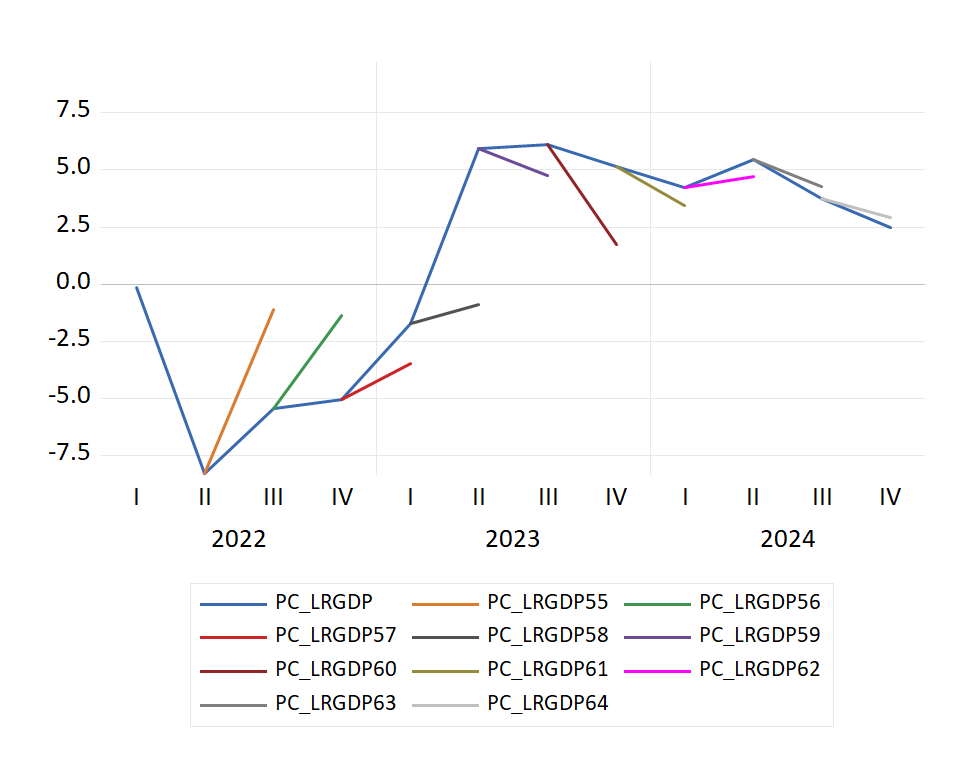
\includegraphics[scale=0.7]{images/image43}
		\caption{Прогноз вневыборочных значений реального ВВП на основе модели MFVAR по всем показателям}
		\label{fig:image43}
	\end{figure}
	
	Из таблицы \ref{tab:metrics-1} и графика (Рис. \ref{fig:image43}) заметно, что модель сильно отклоняется на III и IV кварталах 2022 г., II и IV кварталах 2023 г. Особенно это хорошо отражают квадратичное отклонение SE (Squared Error) и абсолютное отклонение AE (Absolute Error).
	Однако несмотря на это, модель показывает хорошие  прогностические возможности. Например, на более спокойном периоде с I по IV квартал 2024 г. модель отклоняется максимум на 0.76 процентных пункта, что является достаточно хорошим результатом.
	
	В таблице \ref{tab:metrics-1} представлены значения отклонений на каждом шаге. Приведем также таблицу усредненных значений метрик. В таблице \ref{tab:model_metrics} представлены усредненные значения всех отклонений, который позволяют в общем охарактеризовать модель.
	
	\begin{table}[h!]
		\centering
		\caption{Метрики RMSE, MAE и MAPE для модели ВВП на основе MFVAR}
		\begin{tabular}{lccc}
			\toprule
			\textbf{Model} & \textbf{RMSE} & \textbf{MAE} & \textbf{MAPE} \\ 
			\midrule
			MF-VAR & 3.106951 & 2.375936 & 51.945069 \\ 
			\bottomrule
		\end{tabular}
		\label{tab:model_metrics}
	\end{table}
	
	Коэффициенты модели MFVAR мы не можем никак интерпретировать. Поэтому для изучения свойств MFVAR модели следует использовать функцию импульсных откликов. Построим функцию импульсных откликов для данной модели, используя разложение Холецкого. На Рисунке \ref{fig:image44} представлены графики откликов темпов прироста ВВП на импульсы остальных показателей в модели. Нас интересуют конкретно отклики темпов прироста ВВП, поскольку мы хотим интерпретировать, как модель организовывает взаимосвязь между ВВП и остальными показателями. Поскольку модель MFVAR представляет каждую высокочастотную переменную в виде трех низкочастотных переменных, то в данном случае мы рассматриваем отклик темпов прироста ВВП на каждый из месяцев каждого показателя в текущем периоде.
	
	\begin{figure}
		\centering
		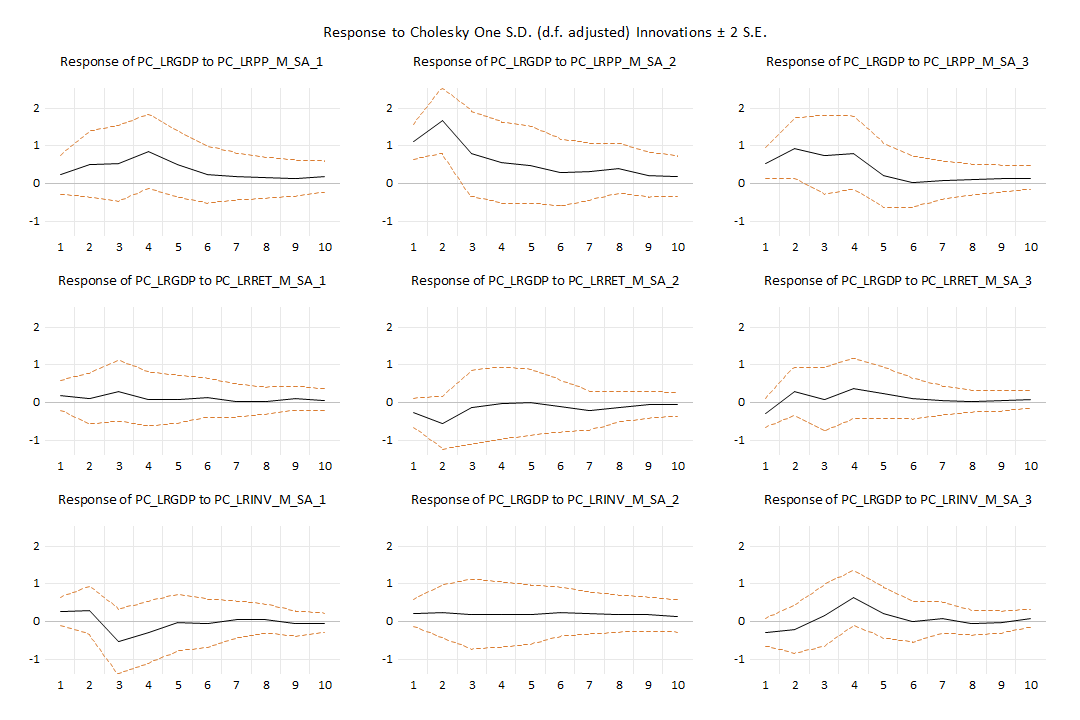
\includegraphics[width=\textwidth]{images/image44}\\
		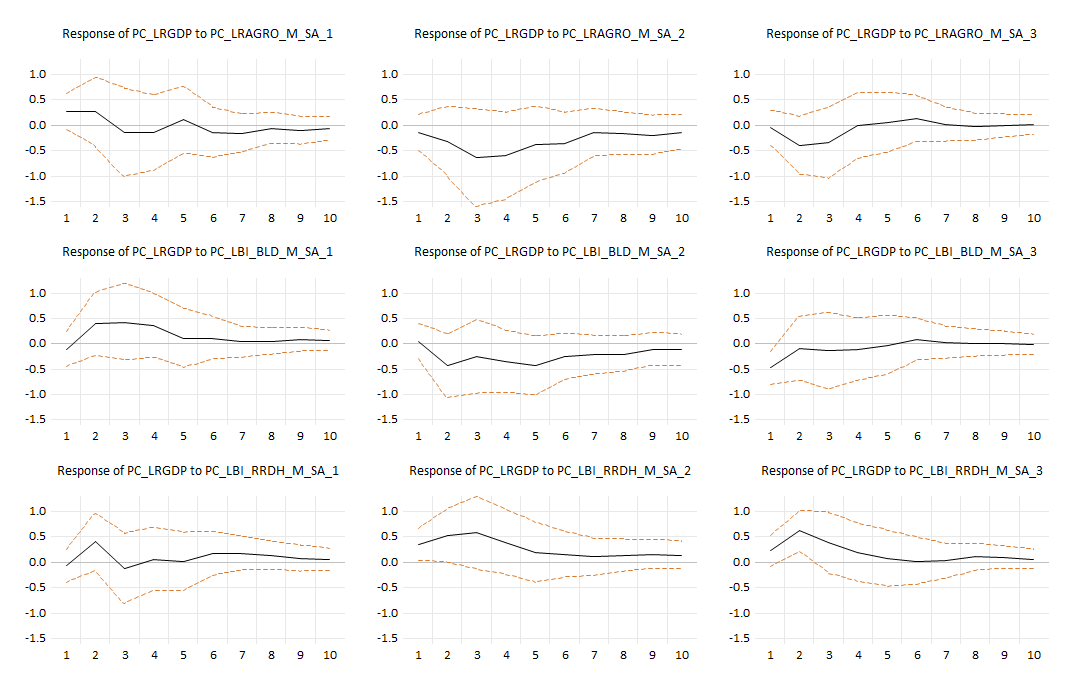
\includegraphics[width=\textwidth]{images/image45}\\
		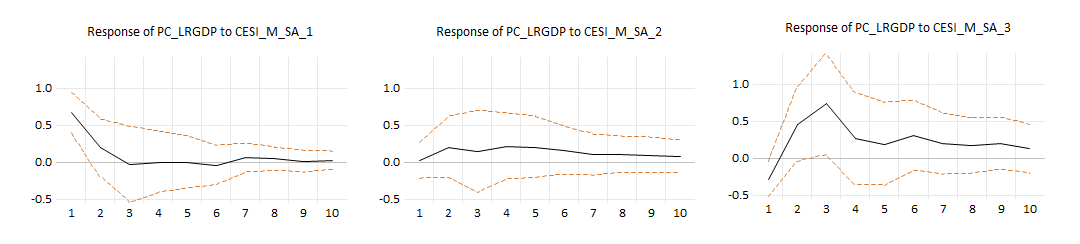
\includegraphics[width=\textwidth]{images/image46}
		\caption{Графики откликов прироста ВВП на импульсы  для модели ВВП на основе MFVAR}
		\label{fig:image44}
	\end{figure}
	
	Из графиков импульсных откликов можно сделать следующие выводы:
	\begin{itemize}
		\item есть возможно незначимый положительный отклик ВВП на импульс первого месяца промышленного производства;
		\item есть значимый в первом и втором периодах положительный отклик ВВП на импульсы второго и третьего месяцев промышленного производства;
		
		\item есть возможно незначимые близкие к нулю отклики ВВП на импульсы розничного товарооборота, инвестиций в основной капитал, первого месяца сельского хозяйства;
		
		\item есть возможно незначимые отрицательные отклики ВВП на импульсы первого, второго и третьего месяцев сельского хозяйства;
		
		\item есть возможно незначимые близкие к нулю отклики ВВП на импульсы строительно-монтажных работ;
		
		\item есть возможно незначимые положительны отклики ВВП на импульсы денежных доходов населения; 
		
		\item есть возможно значимый в первом периоде положительный отклик ВВП на импульс первого месяца СИЭН;
		\item есть возможно незначимый близкий к нулю отклик ВВП на импульс второго месяца СИЭН;
		\item есть возможно незначимый положительный отклик ВВП на импульс третьего месяца СИЭН. 
	\end{itemize}
	
	Таким образом, темпы прироста ВВП имеют незначимые отрицательные отклики на сельско хозяйственную отрасль и положительные значимые и незначимые отклики на остальные показатели. В частности, для темпов прироста ВВП значимыми являются отклики на импульсы
	\begin{itemize}
		\item промышленного производства;
		\item СИЭН.
	\end{itemize}
	Действительно, промышленное производство является аппроксимацией той компоненты, которая составляет большую долю от всего ВВП. Индекс СИЭН же имеет достаточно сильную математическую взаимосвязь с темпами прироста ВВП.
	
	Положительные отклики свидетельствуют о том, что имеются значимые правильные взаимосвязи, поскольку все рассматриваемые аппроксимации компонент участвуют в методах расчета ВВП со знаком <<$+$>>. То есть тот факт, что ВВП положительно откликается на положительный единичный шок в показателях действительно соответствует экономическому смыслу показателей. В случае с сельским хозяйством следует понимать, что хоть отклики и отрицательны, но они могут быть статистически незначимы, поскольку в доверительный интервал входит ноль.
	
	Таким образом, на основе рассмотренных импульсных откликов можно заключить, что построенная модель ВВП действительно удовлетворяет экономическому смыслу, заложенному в нее.
	
	В итоге данную модель ВВП на основе MFVAR можно считать адекватной и применимой для краткосрочного прогнозирования квартальных темпов прироста ВВП.
	
	\newpage
	\chapter*{ЗАКЛЮЧЕНИЕ}\addcontentsline{toc}{chapter}{ЗАКЛЮЧЕНИЕ}
	В данной работе была рассмотрена задача прогнозирования компонент ВВП на основе регрессионных моделей MFVAR. В ходе исследования
	\begin{enumerate}
		\item был проведен полный цикл исследования и преобразования моделей временных рядов для приведения к стационарному виду;
		\item были построены модели MFVAR для прогнозирования и оценки темпов роста ВВП Беларуси по его компонентам, таким как объем промышленности, объем товарооборота, сельского хозяйства, объем строительства, объем инвестиций, объем доходов населения;
	\end{enumerate}
	Таким образом, данная работа вносит вклад в развитие методов прогнозирования на основе моделей временных рядов по смешанным данных и
	может быть использована в дальнейших исследованиях и практических применениях в области экономики и финансов.
\end{document}